\documentclass[12pt]{article}
\usepackage[utf8]{inputenc}
\usepackage[portuguese]{babel}
\usepackage[T1]{fontenc}
\usepackage{amsmath}
\usepackage{lscape}
\usepackage{hyperref}
\hypersetup{
    colorlinks=true,
    linkcolor=blue,
    filecolor=magenta,      
    urlcolor=cyan,
    pdftitle={Overleaf Example},
    pdfpagemode=FullScreen,
    }

\urlstyle{same}

\usepackage[skins]{tcolorbox}
\newtcolorbox{myframe}[2][]{%
  enhanced,colback=white,colframe=black,coltitle=black,
  sharp corners,boxrule=0.4pt,
  fonttitle=\itshape,
  attach boxed title to top left={yshift=-0.3\baselineskip-0.4pt,xshift=2mm},
  boxed title style={tile,size=minimal,left=0.5mm,right=0.5mm,
    colback=white,before upper=\strut},
  title=#2,#1
}
\usepackage{graphicx}
\usepackage{amsfonts}
\usepackage{amssymb}
\usepackage{natbib}
\usepackage{xcolor}
\usepackage[left=2.5cm, right=2.5cm, top=2.5cm, bottom=2.5cm]{geometry}
\parindent=0mm
\parskip=3.5mm
\author{Pedro Botelho & Daniel Vitor}

\begin{document}

\begin{titlepage}
\begin{center}
\large

%----------------------------------------
% CAPA
%----------------------------------------

\begin{figure}[!h]
\centering

\includegraphics[width=6cm]{logo.png}
\end{figure}
\vspace{2cm}
\Large PROGRAMAÇÃO ORIENTADA A OBJETOS \par \vspace{2cm}
\large \textit{1º Relatório do Projeto \textbf{Sistema de Gerenciamento de Academias} (SGA)} \\ \vspace{2cm}
\begin{flushleft}
\textnormal{Desenvolvedor: Pedro Henrique \textbf{Magalhães Botelho}}\\ \vspace{0.5cm}
\textnormal{Desenvolvedor: Daniel Vitor \textbf{Pereira Rodrigues}}\\ \vspace{0.5cm}
\textnormal{Orientador: Atílio \textbf{Gomes Luiz}}\\ \vspace{2.5cm}
\end{flushleft}
GRADUAÇÃO EM ENGENHARIA DE COMPUTAÇÃO - 6º SEMESTRE\\ \vspace{2.5cm}
%ORIENTADOR:
QUIXADÁ - CE\\
2022 \par
\end{center}
\end{titlepage}

\tableofcontents
\newpage

\newpage
\pagenumbering{arabic}

\section{Introdução}

Partindo da proposta para a disciplina de \textbf{Programação Orientada a Objetos}, pelo professor Atílio G. Luiz, é apresentado aqui a idealização do projeto do \textbf{Sistema de Gerenciamento de Academias}, o SGA, como o projeto final da disciplina. 

O projeto partiu de uma proposta mais generalizada e fluiu em uma análise mais específica: construir um sistema simples, porém robusto, que atenda as necessidades de uma pequena academia. Partindo de uma visão simplista uma academia tem alguns pontos que um gerenciamento mais efetivo deve ser usado, tais como: manejar seus alunos, seus funcionários e seu caixa, gerenciando corretamente as mensalidades dos alunos e os salários dos funcionários.

\begin{flushleft}

\textbf{Projeto}: Sistema de Gerenciamento de Academias (SGA)

\textbf{Instituição}: Universidade Federal do Ceará (UFC)

\textbf{Disciplina}: Programação Orientada a Objetos (POO)

\textbf{Desenvolvedores}: Pedro Botelho \& Daniel Vitor

\textbf{Orientador}: Atílio Gomes
\end{flushleft}

\newpage
\section{Descrição do Projeto}

O projeto foca em desenvolver um sistema simples e prático para gerenciamento de pequenas academias, estabelecendo uma relação de simplicidade e robustez. O sistema, a priori, irá realizar o controle do cadastro e dos caixa de alunos e funcionários, utilizando um sistema de banco de dados em arquivo para assegurar a persistência de dados.

Sendo desenvolvido em Java, o sistema, a priori, se utilizará de uma interface de linha-de-comando, também conhecida como CLI, entregando uma interface fácil de usar para o usuário. 

O sistema deverá ser encapsulado em um executável .JAR, de forma que fique mais fácil a inicialização do sistema pelo cliente, sendo necessário apenas clicar duas vezes no lançador, e, como não será utilizado um sistema de banco de dados com servidor local, como MySQL, também não será necessário realizar mais passos.

O sistema tem, atualmente, 6 classes concretas, sem contar a classe principal da aplicação e os enums, que modelam algo dentro do sistema, tal como a empresa da academia, alunos, funcionários, e os gerenciadores. Falaremos em breve sobre eles. 

Os alunos, bem como os funcionários e o próprio banco de dados, serão gerenciados por classes próprias, as classes gerenciadoras, que irão manejar a folha de pagamento e as mensalidades, bem como manter os conjuntos de funcionários e alunos, de forma a construir um banco de dados da empresa. A empresa é modelada por uma classe especial, que guarda as principais informações da academia. 

O sistema ainda conta com um mecanismo de mensalidade sem folga. Isso quer dizer que a situação do aluno irá ficar "em atraso" assim que chegar o dia de sua mensalidade vencer.

\section{Recursos do Sistema}

O sistema deverá ter os recursos essenciais para realizar as tarefas básicas da parte administrativa de uma academia, tais como gerenciar alunos e o caixa. 

Vejamos alguns recursos do sistema:

\begin{itemize}
    \item Modelagem da empresa e Gerenciador de Caixa
    \item Cadastro e gerenciamento de Alunos
    \item Cadastro e gerenciamento de Funcionário, com cargos especificados por um Enum
    \item Sistema de Mensalidade sem Folga
    \item Gerenciamento de Banco de Dados local
\end{itemize}

\section{Planejamento}

Como já dito, o sistema foi desenvolvido em Java. Já o diagrama UML foi totalmente projetado em PlantUML, pois oferece uma interface muito robusta e simples para se desenhar diagramas UML via código.

O projeto foi pensado partindo do "pessoal": alunos e funcionários. "Como representar da melhor maneira possível os objetos que movimentam a empresa?". Depois, foi pensado na parte financeira, isto é, como organizar o caixa da empresa. Dividi-lo em duas partes, onde cada uma irá gerenciar um dos objetos centrais foi a solução. Ao final foi pensando em como modelar a empresa que usará o sistema, bem como o gerenciador de banco de dados.

O projeto está estruturado em pacotes, utilizando a notação "br.com.sga.pacote", para assegurar a sua organização. Foram utilizados classes abstratas, para assegurar polimorfismo e reúso de código, assim como enuns para a organização.

Foram utilizados vários mapeamentos nas classes, para assegurar rapidez e organização. A classe Aluno mapeia os valores pagos de mensalidade a uma data. Já a classe funcionário mapeia os valores pagos de salário a uma data. Caso nulo o pagamento não foi realizado. O mesmo vale para as classes gerenciadoras, que mapeiam um funcionário, ou aluno, para a sua situação quanto ao mês corrente. Essas classes de gerência se baseiam na classe "GerenciadorCaixa", que irá prover os atributos e métodos para controlar o caixa. A classe Pessoa implementa a interface Comparable, dessa forma exigindo que seus descendentes implementem os métodos requeridos. 

Segue, na próxima página, o diagrama UML do projeto. Vale dizer que, por ter uma grande quantidade de atributos, a representação dos métodos getters e setters, assim como os construtores, teve que ser reduzida ao mínimo para caber no diagrama.

\newpage
\begin{landscape}

\subsection{Diagrama UML}
\begin{figure}[!h]
\centering
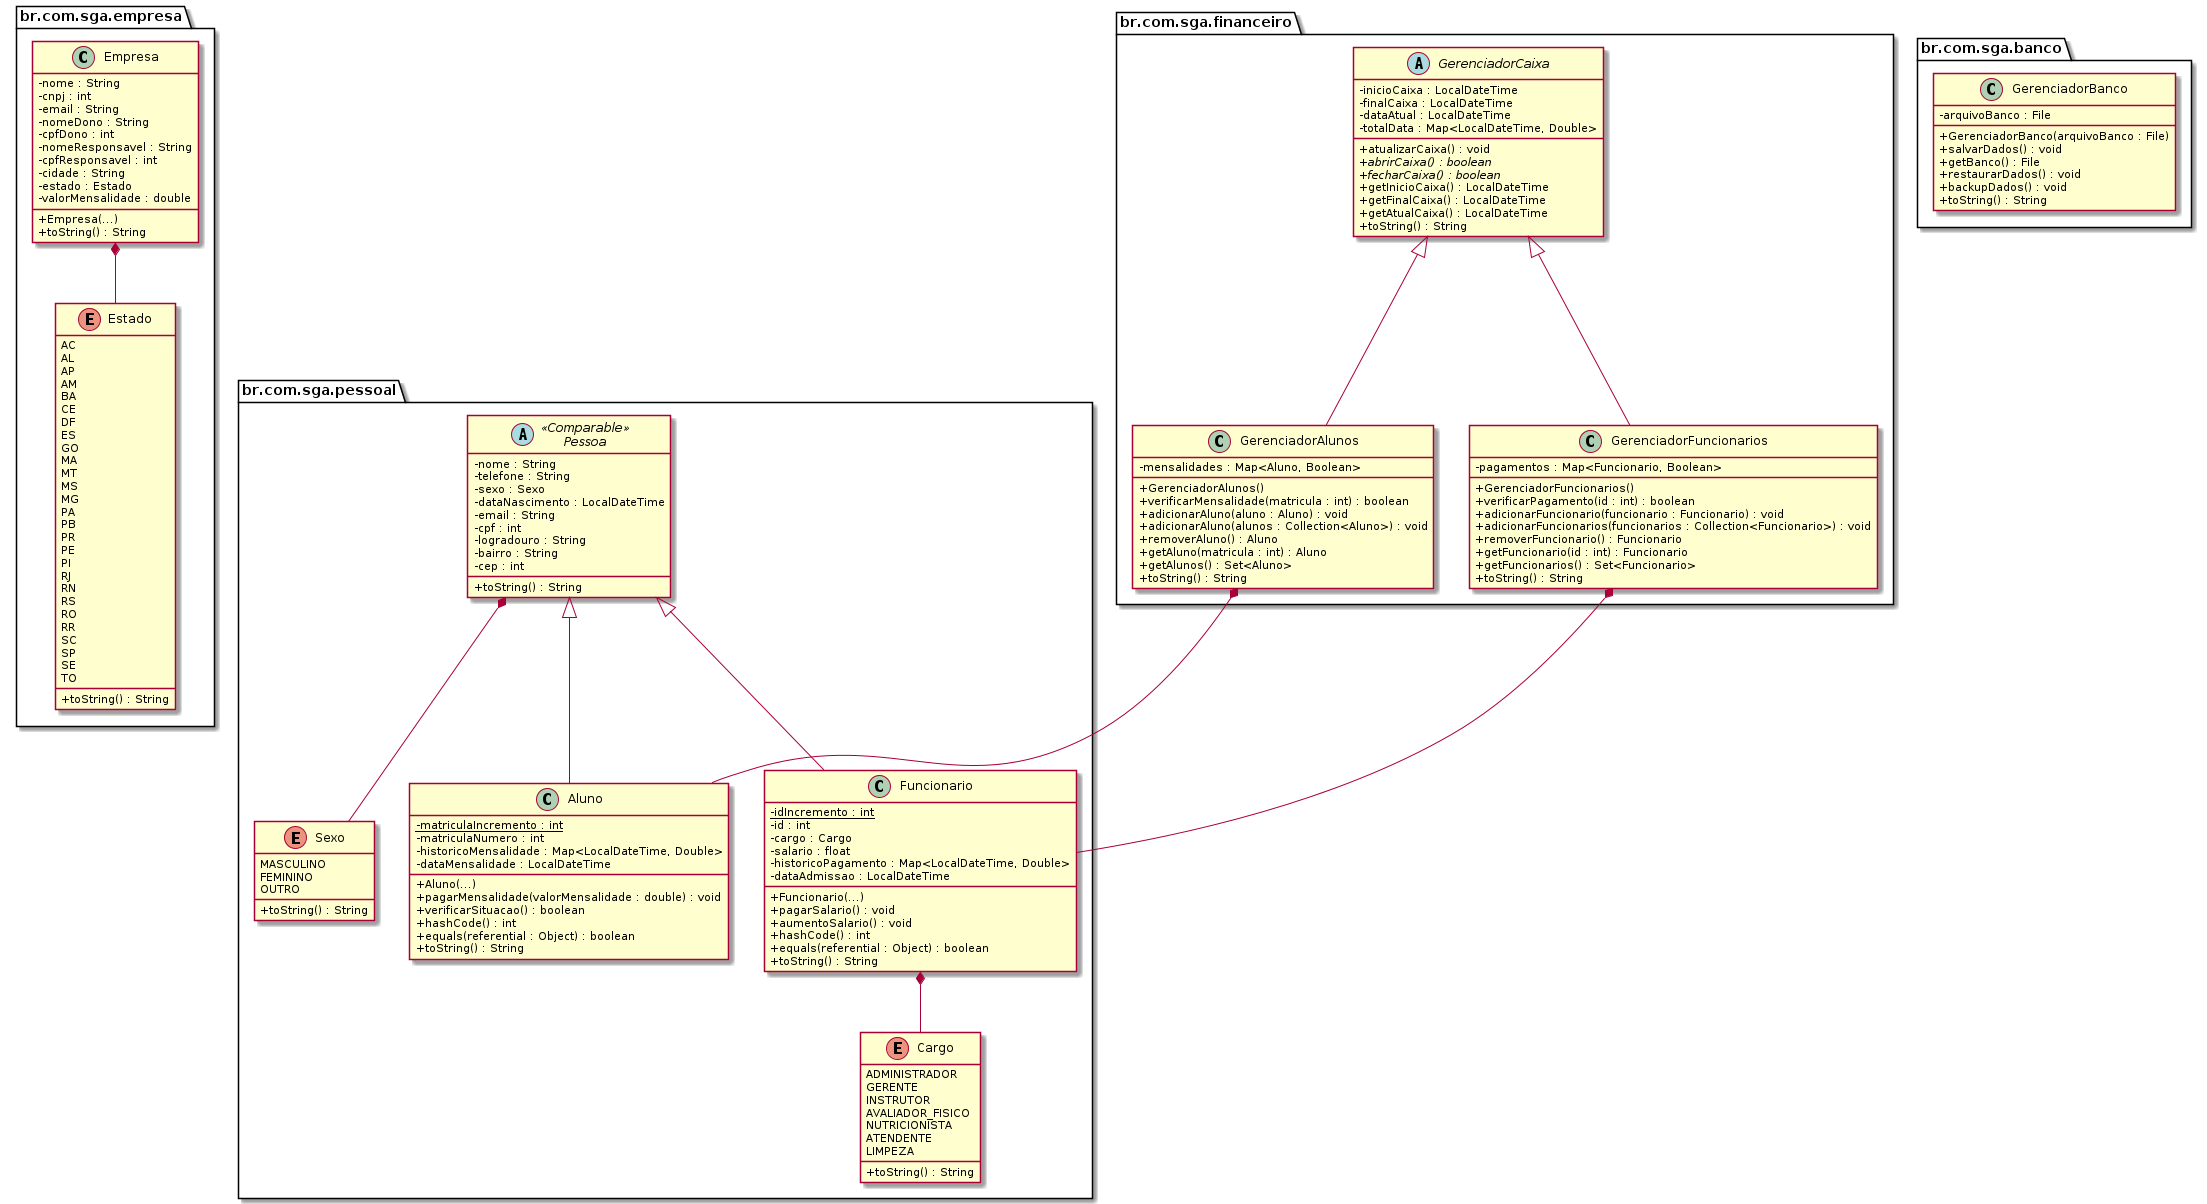
\includegraphics[width=25cm]{sga.png}
\end{figure}
\end{landscape}

\section{Conclusão}

O repositório do projeto pode ser encontrado no
\href{https://github.com/pedrobotelho15/SGA}{GitHub}, tendo toda a estrutura do projeto, bem como o diagrama UML.

\end{document}



